\chapter{Theoretical Appendix A: Model theory and statistical methods}
\label{chap:theoryA}

\section{Model Theory}
\label{modeltheory}
This thesis is concerned with a particular kind of scientific model: those that are subject to mathematical analysis, and tractable subjects for numerical simulation techniques. Most biological models do not fit this description, but increasing computing power has expanded the potential for, in particular, cellular and macromolecular explanations to be formalized and tested in this way. While doing so is sometimes derided as ``physics envy'', the reality is more complex. Simple heuristics are, sometimes, adequate biological explanations; much of differential diagnosis consists of reliable descriptive relations between qualitatively characterised signs in patients, and the presence of a pathogen, for instance. More often, the complexity of biological systems, and the sophistication of the instruments with which we probe them, give rise to observations which support more than one plausible causal explanation for the features of the data. The question of model comparison then immediately arises. Without numerical analysis, we may only make reference to the use of the model in applied domains where the model failure has commercial consequences. Because biological models are rarely required to succeed as engineering tools, for the prediction and control of outcomes of practical significance, an inability to analyse them numerically means that we are left only with rhetoric to assess their relative explanatory value. This approach to ``model comparison'' necessarily devolves into the anarchic Feyerabendian discursive chaos discussed in \autoref{sec:Feyerabend}. Feyerabend correctly points out that scientific models can only be compared against one another, and that the selection of comparative criteria can never be ``objective'' in the sense of being fully independent of the contingent situation and goals of the observer. Nothing can be done about this; either we look for relatively-better criteria and relatively-better models as judged by those criteria, or we remain in the realm of pure metaphysical rhetoric, without investigating their implications, what Feyerabend describes as the realm of the ``crank'':

\begin{longquote}
[T]he distinction between the crank and the respectable thinker lies in the research that is done once a certain point of view is adopted. The crank usually is content with defending the point of view in its original, undeveloped, metaphysical form, and he is not prepared to test its usefulness in all those cases which seem to favor the opponent, or even admit that there exists a problem. It is this further investigation, the details of it, the knowledge of the difficulties, of the general state of knowledge, the recognition of objections, which distinguishes the ‘respectable thinker’ from the crank. The original content of his theory does not.
\cite[p.199]{Feyerabend1981}
\end{longquote}

The support of complex biological systems for multiple explanations gives rise to calls for explanatory pluralism \cite{Brigandt2010}. Very differently parameterised models can be adequate explanations for the same system. This is common for explanations at different descriptive depths. For instance, the models used in \autoref{chap:CMZ} do not descend below cellular level, and make no reference to macromolecules. We would still like to have macromolecular explanations of RPC function, particularly because these may supply us with means to intervene onto RPC proliferative and lineage outcomes, which is a reason to have different models for investigating the molecular phenomena of \textit{rys} in \autoref{chap:rys}.

In other plural explanations, adequate, differently-parameterised models of the same system may be describing different aspects of the same level of organization. Pharmacological kinetic studies of G-protein association with receptors, paired with crystallographic studies of the same phenomenon, supply a good example. These models allow experimenters to pursue different descriptive and interventional objectives. Indeed, as Nicholas Rescher has noted, attempts to synthesize many models into a single overarching explanation often result in descriptive chaos \cite[p.65-6]{Rescher2000}. Rescher argues the adequacy of some model in its domain usually requires the blurring out of at least some pertinent details of the system that could have been included; the computational tractability of the model requires the same.

If we all accept these forms of pluralism, we are still left with the cases where models are making contradictory claims about reality\footnote{That is, they have incompatible metaphysical content; they are therefore subject to counterinduction as mentioned in \autoref{sec:Feyerabend}}. Pluralism cannot coherently extend to abandoning the fundamental logical law of non-contradiction, without compromising the entire endeavour of rationalism. We cannot accept logically contradictory notions about the structure of reality without precluding a broadly consistent view of the way the world works, what Rescher refers to as ``Cognitive Harmony'' \cite{Rescher2005}. Given the complexity of biological systems, we have no option except to express models formally, and to test them rigorously against one another. This is the task of model selection.

Model selection requires that we be able to score models against observations that represent phenomena, to measure their quality. This requires the selection of a quality function. Loss functions, like \hyperref[ssec:AIC]{AIC}, used in \autoref{chap:SMME}, express the relative amount of information in the dataset lost by the model, given a set of parameters. Likelihood functions, used elsewhere, express the credibility of a parameterised model, given the observations. The parameters of the model define an n-dimensional ``parameter space''; the quality function expresses a hypersurface within this space. By sampling within this space, we may estimate the shape of the surface. This sampling information can be used in three ways: we may propose new, higher quality parameter space locations to sample from, in search of the highest quality parameterisation of the model (\hyperref[ssec:MLE]{model optimisation}); we may derive marginal likelihoods for particular parameter values (parameter estimation), or we may estimate the quality of the model over all parameterisations (evidence estimation). These topics are discussed below.

\subsection{Bayesian Epistemological View on Model Comparison}
\label{ssec:BayesEpistemology}
The analyses presented in the data chapters express two views on  model comparison. The first, in \autoref{chap:SMME}, is drawn from information theory, while the second, taken up in \autoref{chap:CMZ}, is a Bayesian view, albeit with more sophisticated tools and more computing power than has been available to Bayesians in the past. In the same way that frequentist analyses may be expressed as a subset of Bayesian analyses (e.g. they seek maximum a priori model parameterisation and likelihood from uninformative priors), informational theoretical approaches to model comparison can be expressed as a subset of Bayesian model comparison theory. In fact, the loss function used in \autoref{chap:SMME}, \hyperref[ssec:AIC]{Akiake Information Criterion}, has been adapted to refer to a prior distribution, as the Bayesian Information Criterion \cite{Posada2004}. The intent of these criteria is to take Occam's Razor to the maximum-likelihood approach, by penalizing the maximum-likelihood value (or maximum a priori score, in the case of BIC) by the number of free parameters.

The general approach of optimizing a model for a quality against a dataset, then penalizing the best model quality by the parameterisation of the model, allows us to overcome an important problem with many maximum-likelihood approaches to model selection: the requirement for models to be parametrically nested. Model nesting precludes \hyperref[sec:Feyerabend]{counter-induction}; we cannot compare models which express fundamentally different views of how the described system is parameterised, only whether adding more parameters improves a particular view. Escaping this limitation allows us to compare stochastic and deterministic mitotic mode models in \autoref{chap:SMME}; these models express different views of how reality is organised. Still, in important ways, this approach shares the basic problem of simply calculating the \hyperref[ssec:MLE]{MLE}: the score does not summarize the robustness of the model fits. That is, a model which is a terrible description of a dataset over most of its plausible parameter space, but an excellent one in a tiny region, can appear to be a better explanation than a model which is a broadly good description over the whole parameter space. Simply using the number of parameters to penalize the best model found fails to capture how justified inclusion of those parameters is, by improving the overall likelihood of sampled models.

This leads us to what may be regarded as the completion of the Bayesian view on model selection\footnote{If nested sampling is not \textit{the} completion of the Bayesian system, it is at least \textit{a} complete Bayesian system.}, John Skilling's system of Bayesian inference, \hyperref[ssec:nested]{nested sampling} \cite{Skilling2006,Skilling2012,Skilling2019}. By rearranging the usual presentation of Bayes' rule, Skilling demonstrates how it specifies computational inputs and outputs associated with the activities of model sampling, parameter estimation, and evidence estimation. Bayes' rule is typically written as follows, where $x$ is a logical proposition about the data (e.g. specific values for the cell cycle length and exit rates of the CMZ), and $Pr(a|b)$ denotes the probability of a given b:

\[Pr(x|data) = \frac{Pr(data|x)Pr(x)}{Pr(data)}\]

This can be read aloud as ``the posterior probability of the proposition, given the data, $Pr(x|data)$, is equal to the likelihood of the data given the proposition, $Pr(data|x)$, multiplied by the prior probability of the proposition, $Pr(x)$, and divided by the marginal probability of the data over all such propositions, $Pr(data)$." This gives the impression that the principal task in statistical analysis is the calculation of the marginal posterior distributions over model parameters, and gives rise to the treatment of the marginal probability, $Pr(data)$, as a mere normalizing constant. Skilling rearranges this to put computational inputs on the left, and outputs on the right:

\[Pr(x)Pr(data|x) = Pr(data)Pr(x|data)\]

This shows us that the evaluation of a model consists of supplying a prior probability for the proposition, $Pr(x)$, and a likelihood function, to assess the probability of the data given that proposition, ($Pr(data|x)$). As computed output: (over many propositions $x$), the total evidentiary mass of the data for this model, ($Pr(data)$), as well as the posterior parameter estimates, $Pr(x|data)$. Sample model parameters are drawn from the prior; the likelihood of these propositions about the data are calculated. By accumulating many such samples, the marginal probability of the model over all of these propositions (the evidence for the model) can be estimated. Because these samples may be weighted by their calculated likelihoods and position on the prior, we may also use them to estimate the marginal posterior probabilities of parameters of interest. 

This encapsulates both the numerical procedures involved in model analysis, as well as the epistemological view implied by Bayesian statistics. That is, a model analysis is the joint product of the model and the data, which expresses our belief about the overall evidence for the model ($Pr(data)$)\footnote{ie. a better model gives higher marginal probability to observations than a worse one}, as well as allowing us to estimate the distribution of credibility we should assign to various values for parameters of the model (propositions), $Pr(x|data)$. These are the two fundamental levels on which quantitative measurements of natural systems allow us to make inferences. We may distinguish between models of the systems in a general sense by their evidence, when applied to the same overall dataset. This allows us to counterinductively test contradictory descriptions of the structure of the phenomenon against one another, inferring which is a better map to the territory. The second level of inference is the ranking of propositions for the parameterisation of models achieved by the sampling procedure. This allows us to determine which particular propositions about the system are supported, given the model and observations. Because the posterior distributions need not be unimodal, we can evaluate these modes as separate hypotheses that are supported to varying degrees by the data. An extensive review of the Bayesian approach to model evidence and model selection has been provided by Knuth et al., covering other methods of estimation not touched on here \cite{Knuth2015}.

This view dispenses with interpretations of model selection as being about finding the ``true model'' of reality, or of estimating the actual, objective probabilities inhering in things or processes (a view disputed in \autoref{sec:chance}). Instead, we are guided to focus on the relative quality of models in explaining all of the relevant data we can gather; we may then evaluate the relative quality of specific propositions about the system within those models (i.e., the posterior distributions on model parameters) as we see fit.  

\subsection{Model sampling and optimization}
\label{ssec:MLE}
There are many techniques used to sample the parameter space of a statistical model, given a quality function which scores the model. These techniques have a variety of purposes. Commonly, one wishes to ``optimize'' a model by finding the parameter vector which produces the best objective function result, given some dataset. This is often referred to as Maximum Likelihood Estimation, the product being a Maximum Likelihood Estimate, with MLE used to refer to these interchangeably. \hyperref[ssec:SPSA]{SPSA} is used in this thesis to optimize cell-based models of RPC activity in \autoref{chap:SMME}. The likelihood scores are penalized by the number of model parameters to produce an \hyperref[ssec:AIC]{AIC} score. MLE methods are broadly useful for many applications, with some tuning. SPSA is used in control systems, to maintain the consistency of modelled processes by estimating the inputs most likely to achieve a setpoint, for instance \cite{Zhou2008}. More sophisticated techniques, like \hyperref[ssec:nested]{Nested Sampling}, involve the estimation of the distribution of quality values over the parameter space, rather than focusing solely on estimating the optimal value.

The process of model sampling requires an algorithmic means to generate proposed parameter vectors to be supplied to the quality function. Most effective sampling methods operate by performing an initial sample from some type of prior information\footnote{In the SPSA optimization performed in \autoref{chap:SMME}, this took the form of the original, poorly optimized fit for the stochastic model and a best guess for a related vector for the deterministic model. In subsequent nested sampling analyses, initialization is performed by sampling randomly from a defined prior distribution.}, and then iteratively generating new proposals from these initial ones. This iterative proposal generation forms a chain of linked positions within parameter space. Generally, new proposals are made considering information related only to the last accepted proposal\footnote{Proposal rejection can occur for a variety of reasons, depending on how the parameter space is interpreted. In Galilean Monte Carlo, this occurs if proceeding along the specified velocity vector would produce a proposal less likely than the last one.}. Because the process is ``memoryless'' in the Markovian sense, and involves the iterative generation of models, it is often called Markov Chain Monte Carlo (MCMC).

Many algorithms for proposal generation exist, and the accuracy and efficiency of sampling procedures depends on their properties. Most offer a physical interpretation of the quality surface in parameter space. Random-walk proposal generation, like the original Metropolis-Hastings implementations of MCMC, is often too inefficient to be usable for high-dimensional parameter spaces, and has broadly been replaced by these physical sampling methods. \hyperref[ssec:SPSA]{SPSA}, for instance, is a simple gradient method. New proposals are generated by bracketing an existing sample with a pair of samples that define an $n$-dimensional ``slope'' at the current location. By proposing a new location down-slope, we receive a new sample which is closer to the local optimum, and we may inexorably approach it in this way. Other, more sophisticated interpretations seek to improve on random-walk proposal generation by mechanical interpretations of proposal movement through parameter space, like Hamiltonian Monte Carlo, or thermodynamic interpretations, like simulated annealing \cite{Andrieu2010}. These methods are better suited to the estimation of the distribution of objective function values than an algorithm like SPSA.

In order to ensure the accuracy of any such estimated distribution across parameter space, the algorithm should, ideally, produce proposals in ``detailed balance'', which refers to the physical concept of reversibility found in classical mechanics. The purpose of constraining proposal generation in this way is to guarantee that particular areas of the parameter space are not over- or under-sampled, distorting the final estimate, as a consequence of the manner in which the sampling algorithm generates proposals. \hyperref[ssec:GMC]{Galilean Monte Carlo} has the property of being in detailed balance, although, as \autoref{chap:GMC} demonstrates, this is not a guarantee of accurate evidence estimation.

\subsection{Overfitting}
\label{ssec:overfit}
Overfitting is a common problem in, particularly, frequentist statistical modelling \cite[p.9-11]{Bishop2006}. It can arise from an unjustified excess of model structure relative to the information present in the data. This excess structure allows the model to capture measurement noise in the dataset the model is being scored against. This produces models which appear highly explanatory, but which reflects the particular structure of the measurement errors in the training data better than the overall phenomenon. This problem will typically become apparent in cases of sequential inference; an overfit model will fail to explain new observations as well as it explained previous ones.

A second source of overfitting is the failure to properly account for uncertainty and prior information. For instance, if unidimensional measurements are modelled with a Normal Gaussian distribution, the MLE Normal Gaussian (whose parameters arise from calculating the mean and standard deviation of the measurements, given the assumption of Normality) can be an overfit to the data \cite[p.28]{Bishop2006}. In this simple example, this usually means that the MLE Normal underestimates overly influenced by ``outliers''. This is one case of the general overfitting problem seen in MLE methods \cite{Green2017}. Accounting for available prior information is the best solution to this problem. As this thesis demonstrates, appropriate accounting for our uncertainty about the parameters of the Normal model, and comparison of the Normal case with appropriate alternatives that might better reflect the underlying causal structure that produces the ``problem'' data (in this case, Log-Normal models), both help in producing more accurate estimates of model parameters.
 
\subsection{Simple Stochastic Models}
\label{ssec:SSM}

\begin{figure}
\makebox[\textwidth][c]{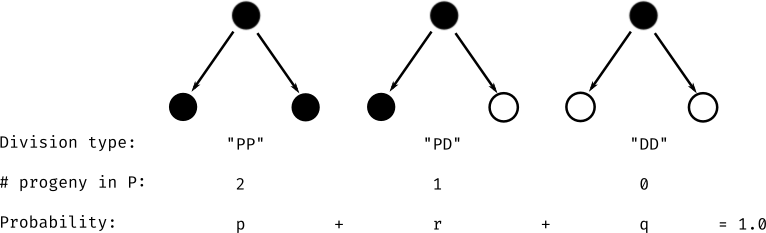
\includegraphics[width=1.\textwidth]{ssm2.png}}    
\caption{{\bf Simple stochastic stem cell model, representing probabilities of cell division events.}} Black circles denote proliferative cells, while white and grey circles denote different types of postmitotic offspring. ``Number of progeny in P" is the number of mitotic offspring produced by each type of division. The probability of each division type must sum to 1, as all possibilities are represented, granting that the division types are defined by the postdivisional mitotic history of the offspring.
\label{fig:SSM}
\end{figure}

The Simple Stochastic Model is schematised in Figure \ref{fig:SSM}. This is the basic structure of the majority of formal models in the stem cell literature, derived from post-hoc analyses of populations taken to include stem and progenitor cells. The population-level approach is usually explicit, as no differentiation is made between types of proliferating cell; in general, no particular cell is identified with a stem cell, nor can any be identified from the necessarily retrospective population data used to infer the parameters of the model. 

The central concept of the model is that mitotic divisions can be categorised by the number of progeny which remain mitotic after the division. This categorisation is necessarily retrospective. This must be kept in mind when considering models of this type, as this categorisation does not necessarily imply that there is some mechanism by which the cell specifies the fate of offspring \textit{at the time of mitosis}, although there is extensive evidence for the coupling of mitotic and specification processes at the molecular level \cite{Tran2013,Tee2014,Dalton2015,Deschamps2017}.

In effect, the model compresses the process of fate specification into individual mitotic events. Since the primary distinction between cells in the model is simply whether they are proliferating or not, the model also elides any heterogeneity within the proliferating population. Beyond not identifying particular cells as ``stem cells", this may make models derived from the SSM inappropriate for proliferative populations with a large degree of heterogeneity. The classic idea of a small number of slowly proliferating ``true" stem cells and a larger population of rapidly dividing ``transit amplifying" progenitors can only be represented by compartmentalised, independent SSMs (as implemented in \autoref{chap:CMZ}).

As Fagan notes, in the SSM, ``relations among p, r, and q values entail general predictions about cell population size (growth, decrease, or ‘steady-state’), and equations that predict mean and standard deviation in population size, probability of [lineage] extinction, and features of steady-state populations are derived."\footnote{While Fagan refers to ``stem cell" extinction, the model does not specifically define stem cells, nor does it imply intergenerational continuity, such that a particular intergenerationally identified stem cell should be said to have become extinct. The unit which survives or is made extinct is the lineage derived from some particular proliferative cell.} \cite[p.60]{Fagan2013}

Typically, this type of model has been employed to describe population dynamics of proliferating cells in assays generating clonal data, where a ``clone" here refers to the population constituted by all offsping descended from some particular (usually ``initial" and sometimes therefore taken for ``stem") proliferating cell. This population is the \textit{lineage} generated by the cell. The mitotic events which give rise to a lineage are summarised as a Galton-Watson branching process, a statistical model originally intended to represent the lineage extinction of surnames. In the case of branching process models applied to proliferative cells, the random variable determines the mode of division of mitosing cells, defined by the proliferative state (construed in the model as being either mitotic or postmitotic) of progeny. For any given division, a cell may produce two mitotic, one mitotic and one postmitotic, or two postmitotic progeny, and each of these division modes is given a defined (often, but not always, static) probability. Given these values, the history of a cell lineage may be simulated; the output of many of these simulations pooled together, in \hyperref[ssec:MonteCarlo]{Monte Carlo} fashion, allows the statistical properties of the dynamics of population of simulated cells to be estimated.

\subsection{Systems of difference equations}
\label{ssec:SODE}
Models defined by difference equations are used in \autoref{chap:CMZ}. A difference equation is the discrete counterpart of a continuous differential equation. Both types of equations can be used to describe the time-evolution of a system, because they can be recursively applied to calculate the value of model outputs at a time $t$, given the value of the outputs at $t-p$, $p$ time units in the past \cite[p.1]{Kelley2001}. In the models presented in this thesis, the simulation's unit of resolution is the day, which motivates the use of the algorithmically simpler analytic solutions to difference equations. As implied above, the time-dependent value of a model output may depend on a output of another equation. This is the case for the model of estimated CMZ annulus population and retinal volume presented in \autoref{CMZoverall}, where the volume estimate depends on resolving the value of the day's starting population before evaluating the volume contribution of that population, given the exit rate. The slice models (see \hyperref[sec:slicemodel]{\path{Slice_Model}}) used to interrogate phase transition timing in \autoref{dvMAPout} are not fully systems of difference equations, since the population difference equation depends on evaluating a continuous power law model of lens growth. Moreover, the slice model of decaying cycle rate (see \hyperref[sec:decaymodel]{\path{Decay_Model}}) depends on the daily evaluation of the continuous exponential cycle time function.

\subsection{Independent Component Analysis models of sequence emission}
\label{ssec:ICA}
The models of \textit{rys} nucleosome position sequence emission presented in \autoref{chap:rys} are products of Independent Component Analysis (ICA), a technique which is used to infer the independent contributions of multiple signal sources on a single multiplex channel; it can be thought of as an application of information theory \cite{Lee2000}. The most common example offered to illustrate this is the separation of the individual streams of speech produced by multiple speakers conversing in a noisy room \cite{Jong-HwanLee2000}. ICA can be used, in this context, to model the process by which a listener separates the independent signals of the speakers from background noises. In this thesis, the \textit{D. rerio} genome is treated in this fashion. In effect, any given sample of genomic sequence may be treated as a multiplex channel produced by a host of independent causal processes. In this sense, each nucleosome position is a ``noisy room'', with its own local structure of background noise and conversational participants. 

The distinction between background noise and signal in an ICA model is made both conceptually, and in the numerical representation of these parts of the model. I have closely followed the early, pioneering example of Down et al. \cite{Down2005}. Down et al. use \hyperref[ssec:HMM]{Hidden Markov Models}, \hyperref[ssec:MLE]{optimized} on promoter sequences, as background models for promoter sequences in general. Against this, a foreground of \hyperref[ssec:PWM]{Position Weight Matrix} signals, representing binding motifs within the promoter region, is inferred by \hyperref[ssec:nested]{nested sampling}. Similarly, in \autoref{chap:rys}, separate HMMs were used to represent genomic sequences from the exonic, ``periexonic'' (introns and $\pm$500bp intervals around the CDS), and intergenic sequences, against which the foreground of repetitive PWM structural signals is inferred, representing characteristic preferred contact points between the core nucleosome and genomic DNA. The HMM background models and $s$ PWM signal models are linked in their description of a set of $o$ observations by an $o \cdot s$ mixing matrix. While many implementations of source and background mixing are possible, in this case, Down et al.'s simple binary implementation is retained. Each observation $o$ is associated with a ``mix vector'' of $s$ binary values, indicating whether or not $s$ source is to be scored in that observation.

The likelihood scoring function for this model is numerically equivalent to Down et al., and is available in full in \autoref{ssec:IPMlikelihood}. Briefly, for every observed sequence whose mix vector indicates a source is present, a score matrix is produced for that source and observation. This involves ``scanning'' the PWM down the length of the observation, offering a score for the entire PWM at each base (in the default reverse-complement operation of \hyperref[chap:BMI]{BioMotifInference.jl}, this is repeated with the reverse complement of the motif, for motif detection on the reverse strand). This feature of likelihood function confers the ``multiple uncounted'' nature of the motif representation in these models. This means that multiple occurrences of a PWM source motif in a sequence can be detected, and that no particular number of occurrences must be specified. These features make this model particularly well suited to the detection of the repetitive structural signals inferred in \autoref{chap:rys}. The PWM source score matrices are subsequently ``woven'' by combination with background scores, an expectation value for motif observation, given the length of the sequence, and a penalty for every source included in the observation, which prevents \hyperref[ssec:overfit]{overfitting}.

\subsection{Position Weight Matrices}
\label{ssec:PWM}
Position weight matrices (PWMs) were used to model signals arising from nucleosome contacts with their DNA positions in \autoref{chap:rys}. For a sequence signal of length $\lambda$, the PWM which defines it is a $\lambda \cdot 4$ matrix, with each of the four columns representing the categorical probability weights of A, C, G, and T\footnote{This base ordering is computationally significant, since it allows for trivial reverse complementing by reversing the matrix values across both dimensions.} base emission at the position represented by row $\lambda$ \cite{Stormo1982}. The PWM is typically used in a frequentist context, without prior distributions over its parameters. However, in a Bayesian context, the PWM is easily interpreted as a $\lambda$-base length vector of discrete categorical distributions over base emission frequencies\footnote{That is, a vector of nonparametric categorical distributions, themselves on a support of ACGT vector of the 4 nucleotide base emission frequencies. \path{BMI.jl} encodes the support as the integers 1234 for computational efficiency}. A computationally useful conjugate prior distribution for discrete categoricals is the Dirichlet distribution \cite{Minka2000}. Vectors of Dirichlets have been used as the priors for signals in \path{BMI.jl} models. Because of their conjugacy, Dirichlet priors can theoretically be updated to produce full posterior distributions over the PWM's parameters. \path{BMI.jl} does not provide for this, for reasons related to the ICA PWM model implementation discussed in \autoref{chap:BMI}. The 4-parameter Dirichlet over the 4-category probability simplex can be usefully thought of as a density cloud in a 3-dimensional tetrahedron (i.e., an ordinary one with 4 vertices). The relative density within the tetrahedron expresses the prior (or posterior) probability of a particular categorical distribution at base $\lambda$. The points of the tetrahedron represent categorical distributions with unit probabilities for one of the four bases, while points in the center of the tetrahedron represent categoricals with identical .25 probabilites of emitting each base. 

\subsection{Hidden Markov Models}
\label{ssec:HMM}
Hidden Markov Models (HMMs) were used to model \textit{D. rerio} genomic background noise in \autoref{chap:rys}. An HMM is a state machine; it can be in one of a finite number of states at any given time. Each state is associated with a probability distribution on the model's emission of symbols. The HMM generates a sequence of such symbols by transitioning from state to state (or remaining in the same state, called autotransition), emitting after each transition. The states are ``hidden'' in the sense that their presence is inferred from the sequence of data upon which the model is trained, and not from direct observations of the states themselves. HMMs are, therefore, well-suited to modelling sequences of outcomes with obscure or irrelevant causal structures. A $k$-state HMM that emits $s$ symbols is defined by an initial state probability vector of length $k$, a $k\cdot k$ state transition probability matrix, and the outcome probability vectors for each state \cite{Rabiner1989}. HMMs can be used in a variety of contexts, each of which is associated with different algorithmic procedures. For instance, the Viterbi algorithm can be used, given an HMM and a sequence of observations, to infer the most likely state the HMM would have resided in at each position in the sequence, had it been generated by that HMM. An example of this use is the inference of exon and intron features from an HMM trained on annotated CDSes \cite{Henderson1997}. In this thesis, HMMs are optimized by an \hyperref[ssec:EM]{Expectation Maximization} algorithm, and are subsequently used to score the likelihood of \textit{rys} sibling and mutant nucleosome position sequences, given their genomic context.

\section{Statistical Methods}

\subsection{Akiake Information Criterion scoring}
\label{ssec:AIC}
An Akiake Information Criterion (AIC) score for a model depends on the number of free parameters in the model, $k$. AIC differences between models can be readily calculated from the residual sum of squares (RSS), which is used as the quality function for measuring model output divergence from observations. For n observations and model parameters $\theta$, $RSS = \sum_{i=1}^{n}(y_i-f(x_i,\theta))^2$. For model comparison, AIC is calculated as:

$mAIC = 2k + n \cdot ln(RSS)$ 
\cite{Burnham2002}

This is not the ``true'' value of AIC but assumes that a constant associated with the same data cancels out during model comparison (i.e. by subtraction). AIC is a flawed model comparison criterion. It takes no account of uncertainty in parameters, and tends to be biased toward simple models \cite[p.33]{Bishop2006}. AIC does not fare well for the evaluation of models whose parameters are not well-constrained by the data \cite[p.217]{Bishop2006}. AIC calculations are implemented in \autoref{ssec:SPSAfix}.

\subsection{Monte Carlo simulations}
\label{ssec:MonteCarlo}
Monte Carlo refers to the repeated sampling of a statistical model's output to estimate quantities related to it. Many of the simulations presented in this thesis involve two distinct uses of Monte Carlo techniques. The first use is the exploration of parameter spaces by Markov Chain Monte Carlo (MCMC), with sequential sampling of locations in parameter space, such that the probability of a proposed new location depends only the current position in parameter space (ie. it is a Markovian trajectory). These proposals can be generated by various means; in this thesis, \hyperref[ssec:SPSA]{Simultaneous Perturbation Stochastic Approximation}, \hyperref[ssec:GMC]{Galilean Monte Carlo}, and \hyperref[ssec:adhoc]{an ad-hoc permutation routine} are used. The second use of Monte Carlo is the estimation of model outcomes distributions, which involves repetitively sampling the same position in parameter space to empirically determine a distribution, against which observations are scored. This is how the majority of the models in the thesis are scored. 

\subsection{Simultaneous Perturbation Stochastic Approximation (SPSA)}
\label{ssec:SPSA}
SPSA is a model \hyperref[ssec:MLE]{optimization technique}. It is a reliable gradient-descent method for finding the local optimum in parameter space, given an objective function and a sample starting position. It has been proven useful in a wide variety of engineering applications \cite{Kleinman1997,Zhou2008}, not least because it is tolerant to measurement noise in the objective function. This makes it useful for applications where exact determination of the measurement function's value is not possible; these include on-line intervention into systems with real measurement noise \cite{Zhou2008}, as well as the calculation of model likelihoods by \hyperref[ssec:MonteCarlo]{Monte Carlo}.

The implementation of SPSA in \autoref{ssec:SPSAfix} follows the example of Spall exactly \cite{Spall1998}, extended with the modifications of Sadegh for bounded parameter spaces \cite{Sadegh1997}, as suggested by Spall. As noted above, SPSA is a gradient-based method. It moves a single model-particle through parameter space. At each iterate, the local quality gradient is estimated by taking two samples on either ``side'' of the particle, given by adding and subtracting a perturbation vector to/from the current location. The perturbation vector is composed by random selection of positive and negative magnitudes in each model dimension. This is ``Simultaneous Perturbation'', the alternative being to perturb dimensions one at a time, which the technique Finite Difference Stochastic Approximation (FDSA) does, instead. SPSA is more accurate and efficient, especially for high-dimensional problems \cite{Chin1997}. Given the quality estimates at the two bracketing samples, the model-particle's position is updated so as to move it downslope (in the case of AIC), toward the local optimum. In order for ever-smaller, higher-quality regions of the parameter space to be consistently found, the distance sampled from the particle for the gradient estimation, and for moving the particle itself, must both consistently decline. This is achieved by tuning coefficients, from which gain sequences are derived. Spall provides useful guidelines on how these may be selected, even automatically \cite{Spall1998}. Experience with the SMME models suggests that a degree of hand-tuning is probably usually necessary.

\subsection{Bayesian treatment of Normal models of unknown mean and variance}
\label{ssec:normalgamma}
As noted in the section on \hyperref[ssec:overfit]{overfitting}, the usual MLE method for characterising a variable population with a Normal gaussian (calculating the mean $\mu$ and variance $\sigma^{2}$) is susceptible to overfitting. In particular, these methods fail to convey the wide uncertainty that usually obtains on the variance parameter of the Normal model \cite{Murphy2007}. Normal models figure heavily in the description of variable population-level data. While these models are well-justified both by their ubiquitous success in parameter estimation, and by information theoretic considerations \cite{Jaynes2003}, and need not reflect the actual distribution of population measures, we use them in this thesis to model these parameters directly. In the main, this is done using LogNormal models, which are Normal gaussians fitted to the logarithm of the data. This change of variable allows more accurate modelling of population data with long right tails, which is common for the outcomes of growth processes. As Heath notes, long right tails are to be expected for values on ranges that are closed at the 0 minimum and open at the high end \cite{Heath1967}. Heath suggests that the Log-Normal distribution should be preferred by default for data of this type. We instead measure the evidence for LogNormal against Normal models for the distributions of our measurements in \autoref{ssec:NormalModels}.

A valid Bayesian means of modeling the credibility of mean and variance parameters on Normal gaussian distributions is the use of Normal-Gamma (NG) prior distributions. This assigns normally distributed uncertainty on $\mu$ and gamma distributed uncertainty on precision, $\lambda$, giving rise to a joint normal-gamma (NG) distribution:

$p(\mu,\lambda) = NG(\mu,\lambda|\mu_{0},\kappa_{0},\alpha_{0},\beta_{0}) \mathrel{\stackrel{\makebox[0pt]{\mbox{\normalfont\tiny def}}}{=}} \mathcal{N}(\mu|\mu_{0},(\kappa_{0}\lambda)^{-1})Ga(\lambda|\alpha_{0},rate=\beta_0)$ \cite{Murphy2007}

In some cases, we have made use of the more convenient Normal-Inverse-Gamma (NIG) distribution, which takes an inverse gamma distribution over the variance $\sigma^{2}$ rather than a gamma distribution over the inverse of variance, $\lambda$:

$p(\mu,\sigma^2) = NIG(\mu,\sigma^{2}|\mu_{0},V_{0},a_{0},b_{0}) \mathrel{\stackrel{\makebox[0pt]{\mbox{\normalfont\tiny def}}}{=}} \mathcal{N}(\mu|\mu{0},\sigma^{2}V_{0})IG(\sigma^{2}|a_{0},b_{0}))$ \cite{Murphy2007}.

These prior distributions have useful properties. One of these is conjugacy; posterior distributions in the same form as the NG or NIG prior may be calculated directly, allowing for sequential inference, although this is not performed in this thesis. Another useful property is that the marginal credibility distribution over the normal model's mean is given by a T distribution, being a weighted sum of an infinite series of Normal distributions with different variances. The marginal distribution of the model mean, calculated from an uninformative NG or NIG prior, is identical to the frequentist Standard Error of the mean \cite{Murphy2007}.

We use the Julia package \path{ConjugatePriors.jl} for the NG and NIG models. However, this package is not provided with functions for fitting these distributions from uninformative priors, nor for calculating marginal distributions. We provide a series of utility functions for these and related tasks in the \path{NGRefTools.jl} package, included in \autoref{NGRefTools}.

\subsection{Empirical Bayes linear regression}
\label{ssec:EmpiricalBayes}
Linear regression models are those that model the response of some dependent variable to a series of independent variables, which are assigned weights. The Empirical Bayes method of linear regression used in \autoref{chap:CMZ} allows the estimation of posterior distributions on the weights, and on the noise of observations about the mean, by specifying the maximum likelihood prior hyperparameters, given the data. Determination of prior distributions from observations is what gives the Empirical Bayes family of methods its name \cite[p.373]{Bernardo2000}. Normally, priors are fixed without reference to the dataset to be examined.

We used the iterative solution to likelihood maximization provided by the analysis of Bishop \cite{Bishop2006}. Briefly, this consists of a series of steps in which $\alpha$ distributions on weights and $\beta$ distributions on the response variable's noise are estimated from the data. This process maximizes the probability of the data $y$ given the $\alpha$ and $\beta$ distributions, over possible values for weights $w$:

$p(y|\alpha,\beta) = \int p(y|w,\alpha,\beta)dw$

Bishop's method naturally produces an estimate of the model evidence, logZ, similar to the more general \hyperref[ssec:nested]{nested sampling}, albeit without an estimate of the error in the evidence.

\subsection{Galilean Monte Carlo}
\label{ssec:GMC}
Galilean Monte Carlo (GMC) is an algortihm for the \hyperref[ssec:MonteCarlo]{sequential Monte Carlo} generation of new sample proposals within a parameter space. While GMC was introduced in 2012 \cite{Skilling2012}, the algorithm used in \path{GMC_NS.jl}, presented in \autoref{chap:GMC}, is Skillings' 2019 revision \cite{Skilling2019}, which prevents model-particles from leaving the likelihood contour in order to find a reflection, and adds an additional reflection direction. 

GMC operates by assigning model-particles (ie. a particular parameterisation of that model at some point in parameter space) a velocity vector, chosen isotropically (ie. uniformly, without preference for any direction). New proposals are generated by moving the particle along the velocity vector. A proposed position's likelihood is calculated, and the proposal is accepted if this value is greater than or equal to the contour. Equality is required to allow particles to search flat likelihood "plateaus", which are prominently seen in the models of \path{CMZNicheSims.jl}, presented in \autoref{chap:CNS}, due to the discretised (timepoint-bound) nature of the observations.

If a proposal is rejected, its current vector crosses the likelihood contour at a distance less than that of the proposal. If this occurs, the particle reflects off the boundary and carries on down the reflected vector with the same velocity. Unlike MCMC methods that rely on differentiating the likelihood surface, in GMC, nothing about the underlying surface is used to propose positions, so it samples evenly from within the likelihood contour, fulfilling detailed balance \cite{Skilling2012}. This means that particles are equally likely to transition between positions in the forward process as the reverse process; in GMC the proposal process to move up-vector is identical to the one to move down vector, eg. a particle reflecting normal to the boundary.

\begin{figure}[!h]
    \makebox[\textwidth][c]{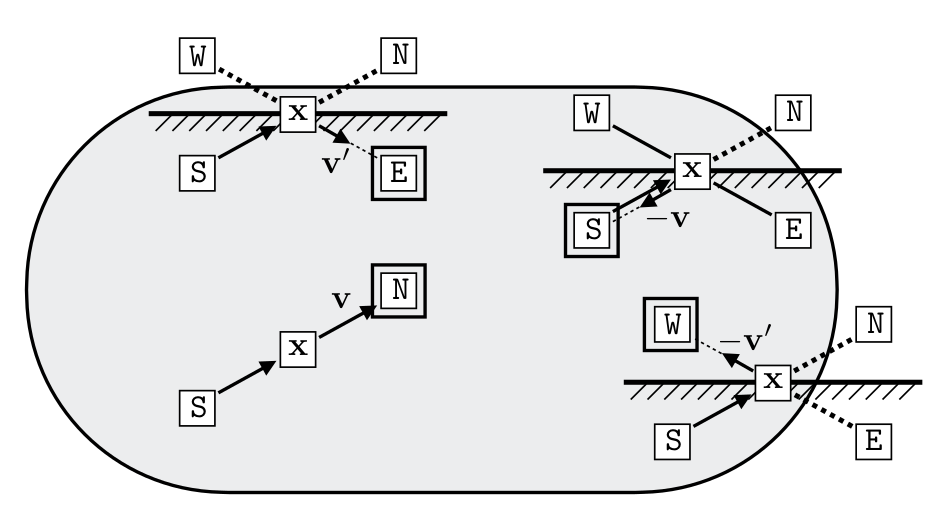
\includegraphics[width=.7\textwidth]{GMC.png}}    
    \caption{{\bf The four directions of GMC particle movement.}} "North" is forward movement along the trajectory; East, South ,and West are reflected vectors. Excerpted from \cite{Skilling2019} under CC-BY 4.0.
    \label{GMCfig}
\end{figure}

When a reflection is being proposed, samples are sequentially taken in three ``directions'', with the first of these to fall within the likelihood contour used as the reflected model-particle. A schematic summary of this scheme is presented in \autoref{GMCfig}. The orientation of the likelihood boundary is inferred by the difference in likelihood between the current particle position and the forward position outside the contour, which is used to estimate a normal vector. The ``east'' reflection is calculated first, followed by the ``west'' reflection, which uses the reversed reflection vector, followed by the ``south'' reflection, which reverses the particle velocity rather than relying on the boundary normal estimate. In \hyperref[chap:GMC]{\path{GMC_NS.jl}}'s implementation, each time a forward or reflected model is rejected because it is outside the likelihood contour, this is logged in the particle's PID tuner memory, which reduces the timestep for another round of forward, east, west, and south searches. Eventually, if no new model can be found above the ensemble's minimum timestep, the particle's trajectory is terminated.

\FloatBarrier

\subsection{Nested sampling}
\label{ssec:nested}
Nested sampling is an algorithmic process for estimating the quality of a model, given observations. It arises from fundamental considerations of imposing a measure on statements about a model of a phenomenon \cite{Skilling2012}. The most basic such statement is an atomic true/false proposition. A measure is a function that assigns a value to a set. A measure of a model's evidence values a statement or a set of statements about the model, given some observations. A set of statements about the model can be represented as a boolean lattice of the statements and their OR combinations \cite{Knuth2012}. The sum and product rules arise in combining measures assigned to these statements into measures of their sets: ie. the probability of A OR B is $p(A) + p(B)$, while the probability of A AND B is $p(A) \times p(B)$. These operators are required in order to preserve consistent ordering between measures and their combinations. This lattice-oriented view thus gives rise to a unique calculus for measuring the divergence of model output from observations over sets of model-propositions\cite{Knuth2012}. This calculus of divergence leads naturally to the concept of information \cite{Skilling2012}, which can be understood in a nested sampling context as related to the compression ratio of the final posterior sample on the prior\footnote{Information, H, is the negative logarithm of the compression ratio. \cite{Skilling2006}}. Moreover, it allows the measure of the total quality of the model, given data: Bayesian evidence or logZ. The uniqueness, basic symmetry, and non-arbitrary nature of the axioms underlying nested sampling strongly suggest that this approach is fundamentally superior to other, more ad hoc methods of estimating model quality (eg. \hyperref[ssec:AIC]{AIC}). While nested sampling can use any quality function, normally a measure of likelihood is used.

The most basic nested sampling procedure involves initialising an ensemble of model-particles by sampling evenly from prior distributions on their parameters. Given this initial ensemble, ``learning'' is performed by compression, where the least likely particle is removed, and replaced by one from inside the likelihood contour established by the least likely particle. Over many such iterates, the ensemble of model-particles is compressed into more and more likely areas of the parameter space. These samples allow us to reconstruct the posterior from their likelihood-weighted parameter locations. More importantly, they allow the estimation of the Bayesian model evidence for the dataset.

Integrating under the quality surface of the parameter space is likely to be an intractable problem for high-dimensional models. However, the dimensionality of the problem can be reduced. If the samples are considered solely in terms of the amount of prior mass enclosed within their likelihood contour, and the likelihood itself, the problem becomes a two-dimensional integration. To do this, the samples taken from the ensemble must be put in order from least to most likely (hence the requirement for consistent ordering in the underlying quality measure, mentioned above). Nested sampling produces this ordering by removing the least likely particle from the ensemble with each iterate. A schematic of the evidence integration is displayed in \autoref{nestedfig}.

\begin{figure}[!h]
    \makebox[\textwidth][c]{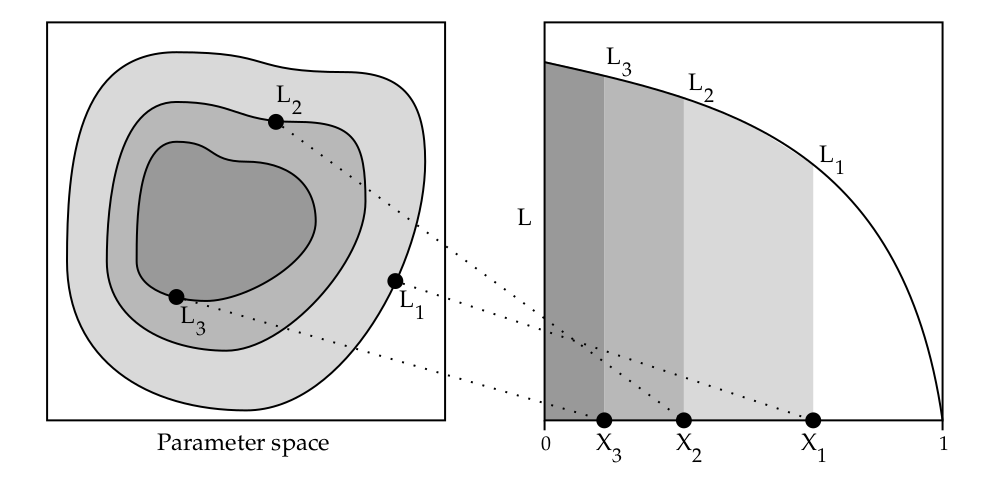
\includegraphics[width=.7\textwidth]{nested.png}}      
    \caption{{\bf Schematic of evidence integration by nested sampling.}} L, likelihood. X gives the fraction of prior mass remaining. Excerpted from \cite{Skilling2006}, copyright John Skilling.
    \label{nestedfig}
\end{figure}

Both samplers implemented in this thesis use the common crude approximation of the sequence of enclosed prior mass values, distributed along the X axis in \autoref{nestedfig}. In this approximation, the fraction of prior mass enclosed by iterate $i$ in an ensemble of $N$ particles is given as $X_{i}=exp(-i/N)$ \cite{Skilling2006}. Very accurate samplers use this approximation to good effect, including MultiNest \cite{Feroz2009}. Having an estimate of the prior mass enclosed at each iterate allows us to determine how much of the prior lies between two iterates by subtracting the inner contour's enclosed mass from the outer\footnote{\path{GMC_NS.jl} and \path{BMI.jl} both use a trapezoidal approximation of the shell width, rather than simple subtraction, although the difference this makes to the evidence estimates is slight.}. Doing so estimates the width of the prior between the two iterates. Multiplying the iterate's sampled likelihood by its prior width gives an estimate of the mass of the evidence between these two contours. Summing the logarithm of the masses of these nested shells between iterates estimates the model evidence, logZ. As Skilling notes, this value is not dimensionless, but rather has data units \cite{Skilling2012}. That is, the logZ value depends on the observations supplied to the likelihood function. However, by taking the evidence ratio between models (by subtracting one evidence value from another), we produce a dimensionless quantity, logZR. This expresses the extent to which the data favour one model over the other (a logZR of 0. would indicate the models are equally credible in light of the data). The uncertainty of logZ values, and hence logZR, are available by using the information, $H$ of the ensemble. This uncertainty is estimated as $\sqrt{H/N}$ for an ensemble of $N$ particles. The uncertainty of a logZR value allows us to express the crediblity range of the logZR estimate as a measure of significance. We calculate standard deviations $\sigma$ of significance by taking the ratio of the uncertainty over the absolute value of logZR. This suggests the probability that the logZR ratio includes 0., indicating equal credibility of the models, assuming normally distributed errors. For instance, a 3 $\sigma$ significance on a logZR value indicates a 99.7\% probability that the favoured model in fact has greater model evidence than the disfavoured model.

\subsection{Expectation-Maximization optimization of HMMs}
\label{ssec:EM}
To select background models for \textit{D. rerio} genomic noise in \autoref{chap:rys}, \hyperref[ssec:HMM]{HMMs} must be \hyperref[ssec:MLE]{optimised} against samples of genomic sequences. HMMs are initialised from prior distributions on their parameters. The prior on symbol emission is usually uninformative. However, because the genomic features we wish to capture with these models consist of runs of bases with particular nucleotide biases, we supply a prior favouring larger values for the transition matrix diagonal, making autotransition (state residency) more probable. Once models are initialised, new model-proposals are generated by iterating expectation-maximization algorithm steps on the HMM. EM algorithms monotonically produce more probable models with every step \cite{Rabiner1989}, without any models being rejected. However, they are generally thought to be susceptible to models getting ``stuck'' at saddle points and in local minima, although EM algorithms will reliably find global optima for some HMMs, under certain conditions \cite{Yang2015b}. It is also possible to use \hyperref[ssec:MonteCarlo]{Markov Chain Monte Carlo} to perform this task, although doing so requires a carefully constructed sampler \cite{Ryden2008}.

Expectation-maximization algorithms work by iteratively cycling through (E)xpectation and (M)aximization steps. In the E step, the most likely hidden states of the HMM, given the observations, are calculated. In the M step, the model parameters are set to those that make the inferred hidden state sequences most likely. More than one way of calculating these quantities is available. \path{BioBackgroundModels.jl} implements the classic Baum-Welch (BW) algorithm \cite{Baum1966}, closely following Rabiner \cite{Rabiner1989}, with the corrections for errata in multiple observations calculation provided by Rahimi \cite{Rahimi}. It also implements the linear memory algorithm of Churbanov et al., \cite{Churbanov2008}. 

As the name suggests, the Churbanov algorithm's memory use increases linearly with the number of HMM states, while BW's increases geometrically. This arises from the different way in which the calculations are performed. For $O$ observations of $T$ length, a $K$-state HMM requires an array of $O \cdot T \cdot K_i \cdot K_j$ to calculate $\epsilon$s, which are the probabilities of being in states $i$ and $j$ at subsequent times, given the model and observations. Memory use increases over the length of the observations vector, resulting in large spikes of memory use over the course of the E-M iterte. The relevant code is found in \autoref{ssec:BaumWelch}, line 26. For large (genome-scale) O and T, memory use on $\geq6-K$ HMMs is prohibitive, especially if more than one model is being learnt on the same machine. By contrast, the Churbanov algorithm cumulates the relevant probabilities using two $O \cdot K_i \cdot K_j \cdot K_m$ arrays, representing the marginal probability of all state paths emitting the observed sequence, that pass through an $i$-$j$ transition at least once, and terminate in state $m$. These two arrays are the memory commit for observations of any length (i.e. there is no $T$ dimension). The relevant code in found in \autoref{ssec:Churbanov}, line 12. Usually, this represents a trivial memory commitment, and longer observations do not increase it. Theoretically, this algorithm can be used to learn HMMs on sequences of any length, unlike standard BW. Although the linear memory algorithm is theoretically less performant than BW \cite{Churbanov2008}, our implementation benchmarks faster than BW in most realistic observation sets. BW may be more appropriate for small numbers of short observations, but Churbanov should usually be the first choice for learning background models on large samples of genomic sequence.